\documentclass{article}
\usepackage{graphicx}
\usepackage{amsmath}
\usepackage{amssymb}
\usepackage{mathtools}
\usepackage{mathrsfs}
\usepackage{titletoc}
\usepackage{tikz}
\usepackage{fourier-orns}
\usepackage{fancyhdr}
\usepackage{booktabs}
\usepackage{array}
\usepackage{easytable}
\usepackage[margin=1cm]{geometry}
\usepackage[most]{tcolorbox}
\usepackage{hyperref}
\hypersetup{
    colorlinks=true,
    linkcolor=blue,
    filecolor=magenta,
    urlcolor=cyan,
    pdftitle={Distributions of Brownian Motion},
    pdfpagemode=FullScreen,
}
\urlstyle{same}
\newcommand{\R}{\mathbb{R}}
\newcommand{\BAB}{\mathbb{\big\vert}}
\newcommand{\NN}{\mathbb{N}}
\newcommand{\Ss}{\\ \vspace{2mm}}
\newcommand{\NL}{\newline
\newline}
\newcommand{\EX}{\mathbb{E}}
\newcommand{\PR}{\mathbb{P}}
\renewcommand{\headrule}{%
\vspace{-8pt}\hrulefill
\raisebox{-2.1pt}{\quad\decofourleft\decotwo\decofourright\quad}\hrulefill}
\geometry{
    left=1cm,
    top=1in,
    right=1cm,
    bottom=1cm
}

\fancyhf{}
\newcommand{\papertitle}{Distributions of Brownian Motion \& Continuous-Time Stochastic Processes}
\fancyhead[LE]{\thepage}
\fancyhead[RE]{\papertitle}
\fancyhead[LO]{\papertitle}
\fancyhead[RO]{\thepage}

\begin{document}
\pagenumbering{gobble}
\begin{titlepage}
    \begin{center}
        \hspace{0pt}\\
        {\scalebox{2}{\Huge\bfseries DISTRIBUTIONS}}\\
        \vspace{4mm}
        {\scalebox{2}{\Huge\bfseries OF BROWNIAN}}\\
        \vspace{4mm}
        {\scalebox{2}{\Huge\bfseries MOTION}}\\
        \vspace{4mm}
        {\scalebox{2}{\Huge\bfseries CONTINUOUS-TIME}}\\
        \vspace{4mm}
        {\scalebox{2}{\Huge\bfseries STOCHASTIC}}\\
        \vspace{4mm}
        {\scalebox{2}{\Huge\bfseries PROCESSES}}\\
        \vspace{0.8cm}
        {\Large\bfseries PROFESSOR ROBERT WEBBER}\\[5pt]
        \vspace{4mm}
        {\Large\bfseries TRISTAN ENDO}\\[5pt]
        \vspace{3mm}
        \begin{figure}[h]
            \centering
            \includegraphics[width=0.4\linewidth]{UCSD seal.png}
        \end{figure}
        \vfill
        University of California, San Diego\\
        United States---2025
    \end{center}
\end{titlepage}
\pagestyle{empty}
\tableofcontents
\pagebreak
\pagestyle{fancy}
\pagenumbering{arabic}
\setcounter{page}{1}

\section{Distribution of Peaks in Fractional Brownian Motion on [0,1]}

\begin{tcolorbox}[colback=white, colframe=black, boxrule=1pt]
\textbf{
A fractional Brownian motion $X(t)$ is a mean zero Gaussian process on $\{t\in \R :t\geq 0\}$ that has covariance function
\begin{align*}
    \kappa(t_1, t_2)=\frac{1}{2}\Big[t_1^{2H}+t_2^{2H}-\Big|t_1-t_2\Big|^{2H}\Big]\qquad \text{for fixed Hurst parameter } H\in (0, 1)
\end{align*}
The fractional Brownian motion with $H=\frac{1}{2}$ is just the regular Brownian motion. Numerically investigate the distribution of the maximum of a fractional Brownian motion restricted to $t\in [0,1]$. How does the distribution change as $H$ ranges from 0 to 1?
}
\end{tcolorbox}
\subsection{Definitions}
\textbf{Standard Brownian Motion: } Standard Brownian Motion is a continuous-time stochastic process $(X(t),t\geq 0)$ where 4 conditions are satisfied
\begin{itemize}
    \item $X(0)=0$
    \item If $n\in \mathbb{N}$ and $0\leq t_0<t_1<...<t_n$, then the random variables $X(t_1)-X(t_0),...,X(t)-X(t-1)$ are independent.
    \item $\forall s\geq 0$ and $t > 0$, the random variable $X(s + t)-X(s)$ has a normal distribution with mean 0 and variance $t$.
    \item $X(t)$ is a continuous function of $t$
\end{itemize}
\textbf{Hurst Parameter: }A constant, denoted by $H$, measures the ``jaggedness'' of observed motion, with smoother motion directly proportional to the value of $H$.

\subsection{Historical Background}
Brownian Motion measures random fluctuations over time. More specifically, the movements of particles in fluids. It was first idealized by Robert Brown, a botanist, who observed pollen grains suspended in water and noticed sudden jitters in a zigzag pattern. Over time, mathematicians and physicists began to describe the random movements through mathematical modeling. Louis Bachelier proposed a model for bond prices, which resembles the stock market charts today. In the next two decades, Albert Einstein and Norbert Wiener would mold a rigorous mathematical foundation for Brownian Motion, showing stochastic processes can be constructed on a probability space. But what is the difference between fractional Brownian motion (fBM) vs. its standard counterpart? The key lies in the relation between events from one another. Fractional Brownian motion has dependent time increments controlled by the Hurst parameter. As described in the definition, the value of the Hurst parameter determines the correlation between time and observed movement. Because fBM has the dependence property, we have a nonzero covariance.\\
\\
\subsection{Hurst Parameter vs. Covariance}
Examine what happens to the covariance when adjusting the value of $H$.
\begin{align*}
    \kappa(t_1, t_2)=\frac{1}{2}\Big[t_1^{2H}+t_2^{2H}-\Big|t_1-t_2\Big|^{2H}\Big]
\end{align*}
Set $H=0.25,0.50,0.75$ per trial
\begin{align*}
    \kappa(t_1, t_2)=\frac{1}{2}\Big[t_1^{0.5}+t_2^{0.5}-\Big|t_1-t_2\Big|^{0.5}\Big]
\end{align*}
Choose arbitrary time intervals. Set $t_1=1$ and $t_2=3$
\begin{align*}
    \rho_{0.25}=\frac{\kappa_{0.25}(1,3)}{\sqrt{1^{\frac{1}{2}}\cdot 3^{\frac{1}{2}}}}
\end{align*}
Substitute time values into the covariance equation
\begin{align*}
    \kappa(1, 3)=\frac{1}{2}\Big[1^{0.5}+3^{0.5}-\Big|1-3\Big|^{0.5}\Big]=\frac{1}{2}\Big[1+\sqrt{3}-\sqrt{2}\Big]
\end{align*}
\begin{align*}
    \kappa_{0.25}(1,3)\approx&\frac{1.3178}{2}=0.6589\\
    \kappa_{0.5}(1,3)=1\qquad &  \kappa_{0.25}(1,3)\approx1.6839
\end{align*}
\subsection{Numerical Data Analysis}
\begin{figure}[h]
    \centering
    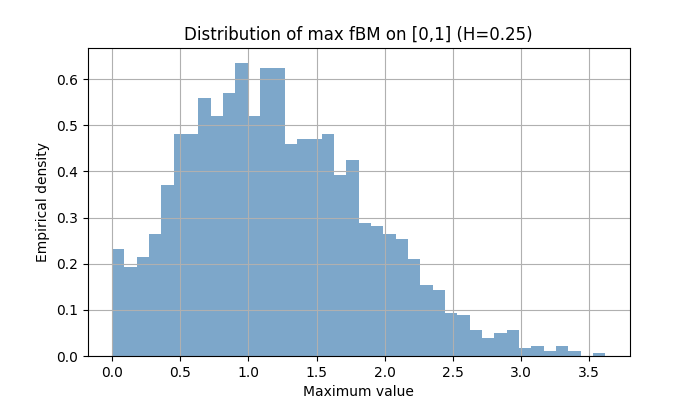
\includegraphics[width=0.5\linewidth]{H25.png}
    \caption{This graph measures the distribution of maxima for $H=0.25$. The maximums are more spaced out but this results in a low maximum because the more samples are wasted not contributing to the maxima count. In this case is only 0.652 (scaled to model empirical density).}
    \label{fig:placeholder}
\end{figure}
\NL
For $H=0.25$, the maximum values tend to be smaller since it is more probable that the trend will change direction at each time jump. From Figure 1, the distribution of maximums is more spread out and this is from the fact that at one time the trend is going one direction and in the next the other. It can be a large value in one time interval, then a really low in the next. Because of this back-and-forth movement, the overall maximum stays relatively small.
\begin{figure}[h]
    \centering
    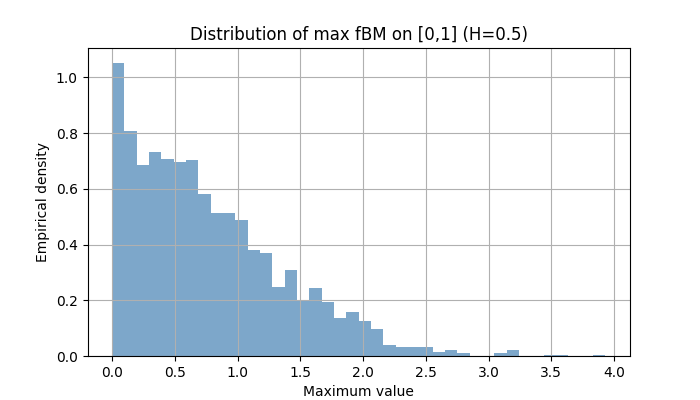
\includegraphics[width=0.5\linewidth]{H50.png}
    \caption{This graph measures the distribution of maxima for $H=0.50$. The maxima are concentrated toward the mean and the extremes are moderately pronounced. There are fewer wasted samples contributing to the maxima count. In this case, the maximum is 1.101 (scaled to model empirical density).}
    \label{fig:placeholder}
\end{figure}
\NL
For $H=0.50$, there is no correlation for the distribution of the maximum. It is equally probable that the trend will either continue or reverse. Thus, the samples will be more condensed in the Gaussian distribution, resulting in higher overall maxima. Notice that the covariance is $0$ when we plug $H=0.5$ and it signifies independence as described in the definition for the standard Brownian Motion.
\NL
\begin{figure}[h]
    \centering
    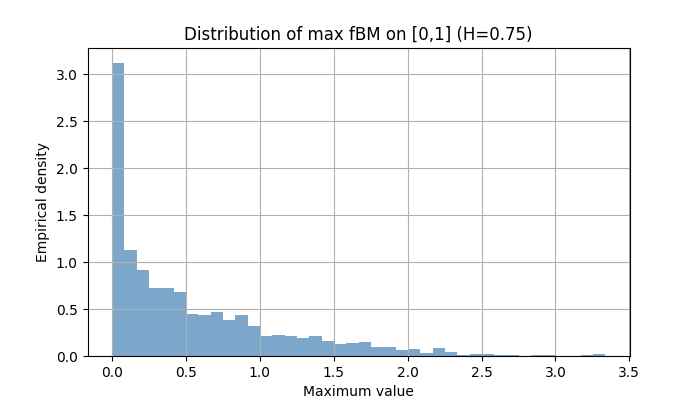
\includegraphics[width=0.5\linewidth]{H75.png}
    \caption{This graph measures the distribution of maxima for $H=0.75$. The maxima are very much concentrated toward the mean and the extremes are greatly pronounced. In this case, the maximum is 3.235 (scaled to model empirical density).}
    \label{fig:placeholder}
\end{figure}
\NL
For $H=0.75$, the strong correlation forces the samples to cluster together in the region of the Gaussian distribution. This results in a lot of samples at or near the mean, more so at the mean. One thing of note is that because of the relatively high Hurst parameter, the samples are more likely to follow the previous sample. This causes the overall maxima to drastically increase, almost triple that of $H=0.50$.
\NL
Using the values calculated for the covariance, solve for the correlation coefficient. The reasoning for this step will be apparent later. For any $t_1$ and $t_2$, in $[0,1]$, the correlation coefficient
\begin{align*}
    \rho_{0.25}=\frac{\kappa_{0.25}(t_1,t_2)}{\sqrt{t_1^{\frac{1}{2}}\cdot t_2^{\frac{1}{2}}}}
\end{align*}
\begin{align*}
    \rho_{0.25}\approx \frac{0.6589}{\sqrt[4]{3}}\approx 0.5007
\end{align*}
The other correlation coefficients for the other Hurst parameters are
\begin{align*}
    \rho_{0.5}=\frac{1}{\sqrt{3}}\approx 0.5773\qquad \qquad \rho_{0.75}\approx0.7389
\end{align*}
Notice that the higher the Hurst parameter, the higher the correlation. But how does the correlation relate to the distribution of the maximum? To test, take some number of samples and count the number of samples that fall into each number bin. There are 40 in total, from $0\to4$ counting by tenths. Because the sampling is only from $t\in [0,1]$, the mean is 0 and the variance is 1. The Hurst parameter measures the concentration of samples toward the mean. The table shows how the maxima count changes as H grows from 0 to 1. It is directly proportional to $H$. Up until this point, $H's$ relation to correlation was never explicit. Here is what the $H$ tells about correlation.
\begin{align*}
    X_H(t)=\begin{cases}
        \text{Positively correlated}& \text{if }H> \frac{1}{2}\\
        \text{Not correlated}& \text{if } H= \frac{1}{2}\\
        \text{Negatively correlated}& \text{if } H< \frac{1}{2}
    \end{cases}
\end{align*}
For $H>0.5$, the Gaussian process is more likely to stay on its trend than divert which the observed motion is seen as more smooth. For $H<0.5$, the Gaussian process is more likely to divert than stay which the observed motion is seen as more spiky. $H=0.5$ is a mixture of both smooth and spiky.
\begin{table}[h]
\centering
\begin{tabular}{|c|c|c|c|c|c|c|}
    \hline
    $H$ & 0.0 & 0.1 & 0.2 & 0.3 & 0.4 & 0.5\\
    \hline
    $\max_{0\leq t\leq1}X_H(t)$ & 0.553 & 0.601 & 0.639 & 0.668 & 0.772 & 1.101\\
    \hline
\end{tabular}
\end{table}
\begin{table}[h]
\centering
\begin{tabular}{|c|c|c|c|c|c|c|}
    \hline
    $H$ & 0.6 & 0.7 & 0.8 & 0.9 & 1.0 \\
    \hline
    $\max_{0\leq t\leq1}X_H(t)$ & 1.690 & 2.836 & 4.224 & 5.607 & 6.800\\
    \hline
\end{tabular}
\end{table}

\pagebreak

\section{Distributions of Standard Brownian Motion and Ornstein-Uhlenbeck Processes}

\begin{tcolorbox}[colback=white, colframe=black, boxrule=1pt]
\textbf{
What is the distribution of Brownian motion $W(t)$ conditioned on observations $W(0)=0$ and $W(1)=x_1$? What is the distribution of an Ornstein-Uhlenbeck process $X(t)$ conditioned on observations $X(0)=x_0$ and $X(1)=x_1$?
}
\end{tcolorbox}
\subsection{Definitions}
\textbf{Ornstein-Uhlenbeck (OU) Process: } An Ornstein-Uhlenbeck process, $X(t)$, is a continuous-time Gaussian Markov Chain that satisfies the stochastic differential equation
\begin{align*}
    dX(t)=\theta\cdot (\mu-X(t))+\sigma \cdot dW(t)
\end{align*}
\begin{center}
    $\theta>0$ is the rate of mean reversion - (how long $X_t$ returns to mean)\\
    $\mu\in \R$ is the long-term mean - the value $X_t$ converges to\\
    $\sigma>0$ is the volatility measure of random fluctuation magnitudes\\
    $W_t$ satisfies all conditions for Standard Brownian Motion
\end{center}
\subsection{Distribution of Standard Brownian Motion}
Let $W(t)$ be Standard Brownian Motion with $W(0)=0$ and for $s,t\in [0,1]$,
\begin{align*}
    \EX[W(t)]=0\qquad \qquad Cov~\Big(W(s),W(t)\Big)=\min(s,t)
\end{align*}
Because $W(0)$, the only quantity to condition on is $W(1)=x_1$. The end goal is to compute the distribution of $\{W(t):0\leq t\leq1\}$.
\NL
Fix a value for $t\in [0,1]$ so that the pair of random variables $\Big(W(t),W(1)\Big)$ is bi-variate normal, where
\begin{align*}
    \EX[W(t)]&=\EX[W(1)]=0\\
    Var(W(t))=t&\qquad  Var(W(1))=1\\
    Cov\Big(W&(t),W(1)\Big)=t
\end{align*}
Apply the properties of conditional distribution $X|Y=y$ for jointly $\mathcal{N}(W(t),W(1))$
\begin{align*}
    \mathcal{N}\Bigg(\EX\big[X\big]+&\frac{Cov\Big(X,Y\Big)}{Var\Big(X\Big)}\Big(y-\EX[Y]\Big),Var(X)-\frac{Cov\Big(X,Y\Big)^2}{Var\Big(Y\Big)}\Bigg)
    \\
    X&=W(t)\qquad \qquad Y=W(1)\qquad \qquad y=x_1
\end{align*}
Find the conditional mean and variance with values defined above
\begin{align*}
    \EX\Big[W(t)~\Big|~W(1)=x_1\Big]&=0+t(x_1-0)=tx_1\\
    Var\Big[W(t)~\Big|~W(1)=x_1\Big]&=t-t^2=t(1-t)
\end{align*}
So that means $\forall t\in [0,1]$, fixed
\begin{align*}
    \Big\{W(t)~\Big|~W(1)=x_1\Big\}\sim\mathcal{N}\Big(tx_1,t(1-t)\Big)
\end{align*}
Divide the time interval $[0,1]$ into $n$ parts so we get sub-intervals $t_1,t_2,...,t_n$ that satisfies $0\leq t_1<t_2<...<t_n\leq 1$. Because $W(t)$ is a Gaussian process, the vector $W$ defined as,
\begin{align*}
    W:=\Big\{W(t_1),W(t_2),...,W(t_n)\Big\}^T
\end{align*}
is also multivariate normal. So we can write $W$ comprised of its mean and covariance. The mean is 0 because of the properties of $W(t)$.
\begin{align*}
    W=\begin{bmatrix}
        \Big\{W(t_1),W(t_2),...,W(t_n)\Big\}^T\\
        W(1)
    \end{bmatrix}
\end{align*}
The covariance matrix is composed for any $i,j\in[1,n]$
\begin{align*}
    Cov\begin{bmatrix}
        X\\
        Y
    \end{bmatrix}=
    \begin{bmatrix}
        \Sigma_{XX}& \Sigma_{XY}\\
        \Sigma_{YX} & \Sigma_{YY}
    \end{bmatrix}   =
    \begin{bmatrix}
        \min(t_i,t_j)& (t_i)_{i=1}^n\\
        (t_i)_{i=1}^n & 1
    \end{bmatrix}
\end{align*}
Compute the conditional distribution of the vector, $W$
\begin{align*}
    X~\big|~(Y=x_1)\sim\mathcal{N}(\Sigma_{XY}\Sigma_{YY}^{-1}x_1,\Sigma_{XX}-\Sigma_{YY}^{-1}\Sigma_{YX})
\end{align*}
Substitute values for each $\Sigma$, and get
\begin{center}
    Mean Vector: $(t_ix_1)_{i=1}^n$\\
    Covariance Matrix: $(\min(t_i,t_j)-t_it_j)_{i,j}$\\
\end{center}
This reinforces the multivariate normal property of the Gaussian Process $W(t)~|~W(1)=x_i$ using the above parameters.
\NL
Now, define another process, $B(t)$, such that
\begin{align*}
    B(t):=W(t)-t\cdot W(1)\qquad 0\leq t\leq 1
\end{align*}
Using the properties of $W(t)$
\begin{align*}
    \EX[B(t)]=\EX[W(t)]=0
\end{align*}
For times $s,t\in [0,1]$,\quad  $\min(1,s)=s,~\min(1,t=t),~Var(W(1))=1$
\begin{align*}
    Cov\Big(B(s),B(t)\Big)&=Cov\Big(W(s)-s\cdot W(1),W(t)-t\cdot W(1)\Big)\\
    &=\min(s,t)-s \min(1,t)-t\min(s,1)+st Var\Big(W(1)\Big)\\
    &=\min(s,t)-st-ts+st\\
    &=\min(s,t)-st
\end{align*}
Note that $B(t)$ and $W(1)$ are independent, which can be deduced by computing the covariance and realizing it equals 0. Thus, rearrange the equation for $W(t)$ and get
\begin{align*}
    W(t)=B(t)+t\cdot W(1)
\end{align*}
It follows that the conditioned process $W(t)~|~W(1)=x_1$ is
\begin{align*}
    W(t)~|~(W(1)=x_1)=tx_1+B(t)
\end{align*}
where $B(t)$ is a Gaussian Process with mean $0$, covariance $\min(s,t)-st$, $B(0)=0$,  $B(1)=0$, and independent of $x_1$. This is the exact definition of the \textbf{standard Brownian Bridge}, which is the distribution of Brownian motion $W(t)$ conditioned on observations $W(0)=0$ and $W(1)=x_1$.

\subsection{Distribution of Ornstein-Uhlenbeck Process}
Let $X(t)$ be an OU Process that satisfies the stochastic differential equation listed in the definition. It follows that the distributions are multivariate normal. In particular, for $s<t$,
\begin{align*}
    \Big(X(t)~\Big|~X(s)=x_s\Big)\sim \mathcal{N}\Big(\mu+(x_s-\mu)e^{-\theta(t-s)},\frac{\sigma^2}{2\theta}(1-e^{-2\theta(t-s)}\Big)
\end{align*}
Now, consider $X(t)$ where $t\in(0,1)$ given $X(0)=x_0$ and $X(1)=x_1$. So, using multivariate Gaussian conditioning,
\begin{align*}
    X(t)~\Big|~(X(0)=x_0,~X(1)=x_1)\sim \mathcal{N}\Big(\mu',\sigma_0^2\Big)
\end{align*}
where $\mu'$ is the conditional mean and $\sigma_0^2$ is the conditional variance, values which need to be computed.
\NL
Start by computing $\mu'$. Recall that the formula for conditional expected value for bivariate normal is
\begin{align*}
    \EX[X~|~Y=y]=\EX[X]+\frac{Cov(X,Y)}{Var(Y)}\cdot (y-\EX[Y])
\end{align*}
Let $Y$ be a $2\times 1$ vector with components $X(0)$ and $X(1)$
\begin{align*}
    Y=\begin{bmatrix}
        X(0)\\
        X(1)
    \end{bmatrix}
\end{align*}
and for quantities involving matrices,
\begin{align*}
    \EX[X~|~Y=y]=\EX[X]+\frac{\Sigma_{XY}}{\Sigma_{YY}}\cdot (y-\EX[Y])
\end{align*}
Here, $\Sigma_{YY}$ is the covariance of $Y$. The reason for the change is the transformation from scalars to vectors, which is a linear transformation from $\R^1\mapsto \R^2$. The matrix formula is required since the general formula only takes inputs in $\R^1$. The conditional mean becomes
\begin{align*}
    \EX\Big[X(t)~\Big|~(X(0)=x_0,X(1)=x_1)\Big]=\\
    \EX[X(t)]+\frac{Cov(XY)}{Cov(Y)}\cdot
    \begin{bmatrix}
        x_0-\EX[X(0)]\\
        x_1-\EX[X(1)]
    \end{bmatrix}
\end{align*}
The value of $\EX[X(t)]=\mu+(x_0-\mu)e^{-\theta t}$. Next, compute the covariance. Note that the process is stationary since we have a fixed starting point $x_0$
\begin{align*}
    Cov\Big((X(t),X(0)\Big)&=\frac{\sigma^2}{2\theta}e^{-\theta t}\\
    Cov\Big((X(t),X(1)\Big)&=\frac{\sigma^2}{2\theta}e^{-\theta (1-t)}
\end{align*}
Combining the two,
\begin{align*}
    Cov\Big((X(0),X(1)\Big)=\frac{\sigma^2}{2\theta}e^{-\theta}
\end{align*}
Putting it all together gives us the mean,
\begin{align*}
    \mu'&=\EX\Big[X(t)~\Big|~(X(0)=x_0,X(1)=x_1)\Big]\\
    &=\mu+e^{-\theta t}\frac{1-e^{-2\theta(1-t)}}{1-e^{-2\theta}}\cdot (x_0-\mu)+e^{-\theta (1-t)}\frac{1-e^{-2\theta t}}{1-e^{-2\theta}}\cdot (x_1-\mu)
\end{align*}
To compute $\sigma_0^2$, employ the conditional variance formula similar to expected value.
\begin{align*}
    Var(X(t)~|~X(0),X(1)]=Var(X(t))-\frac{\Sigma_{XY}}{\Sigma_{YY}}\cdot \Sigma_{YX}
\end{align*}
where $Y$ is defined before as the $2\times 1$ vector. $Var(X(t))$ has already been defined for fixed $X(0)$
\begin{align*}
    Var(X(t))=\frac{\sigma^2}{2\theta}(1-\exp(-2\theta t)
\end{align*}
Additionally, because $X(0)$ is fixed,
\begin{align*}
    Cov(X(t),X(0))&=0\\
    Cov(X(t),X(1))&=\frac{\sigma^2}{2\theta}\Big(\exp(-\theta(1-t))-\exp(-\theta(1+t))\Big)
\end{align*}
\begin{align*}
    \Sigma_{XY}&=\Bigg(Cov\Big((X(t),X(0)\Big),Cov\Big((X(t),X(1)\Big)\Bigg)\\
    &=\Bigg(0,\frac{\sigma^2}{2\theta}\Big(\exp(-\theta(1-t))-\exp(-\theta(1+t))\Big)\Bigg)\\
    &=\Sigma_{YX}\\
    \Sigma_{YY}&=\frac{\sigma^2}{2\theta}\Big(1-e^{-2\theta }\Big)
\end{align*}
Putting it all together,
\begin{align*}
    \sigma_0^2&=Var\Big(X(t)~|~X(0),X(1)\Big)\\
    &=\frac{\sigma^2}{2\theta}\Bigg[\Big(1-e^{-2\theta }\Big)-\frac{\Big(\exp(-\theta(1-t))-\exp(-\theta(1+t))\Big)^2}{1-e^{-2\theta}}\Bigg]
\end{align*}
With $\mu'$ and $\sigma_0^2$ defined, then the conditional distribution
\begin{align*}
    X(t)~\Big|~(X(0)=x_0,~X(1)=x_1)\sim \mathcal{N}\Big(\mu',\sigma_0^2\Big)
\end{align*}
where
\begin{align*}
    \mu'&=\mu+e^{-\theta t}\frac{1-e^{-2\theta(1-t)}}{1-e^{-2\theta}}\cdot (x_0-\mu)+e^{-\theta (1-t)}\frac{1-e^{-2\theta t}}{1-e^{-2\theta}}\cdot (x_1-\mu)\\
    \\
    \sigma_0^2&=\frac{\sigma^2}{2\theta}\Bigg[\Big(1-e^{-2\theta }\Big)-\frac{\Big(\exp(-\theta(1-t))-\exp(-\theta(1+t))\Big)^2}{1-e^{-2\theta}}\Bigg]
\end{align*}
Under conditioning, $Var(X(0))=Var(X(1))=0$. If follows that the OU process is Gaussian and mean-reverting between $x_0$ and $x_1$. This is known as the \textbf{Ornstein-Uhlenbeck Bridge} which is the distribution of an Ornstein-Uhlenbeck process $X(t)$ conditioned on observations $X(0)=x_0$ and $X(1)=x_1$.

\end{document}